\documentclass[10pt,twoside]{ctexbook}
\usepackage[utf8]{inputenc}
\usepackage[T1]{fontenc}
\usepackage{hyperref}
\usepackage{xeCJK}
\usepackage{xeCJKfntef}
\usepackage{listings}
\usepackage{color}
\usepackage{xcolor}
\usepackage{subfigure}
\usepackage{titletoc}
\usepackage{wrapfig}
\usepackage{bm}
\usepackage{fancyhdr}
\usepackage{indentfirst}  
\usepackage{amsmath}
\usepackage{amsfonts}
\usepackage{fancybox}
\usepackage{amssymb}
\usepackage{graphicx}
\usepackage{paracol}
\usepackage{bbm}
\usepackage{bbold}
\usepackage{verbatim}
\usepackage{CJKulem}
\usepackage{ulem}
\usepackage{soul}
\usepackage{tikz}
\usepackage{lastpage} %总页数
\usepackage[left=2cm, right=2cm, top=1.5cm, bottom=1.5cm,a4paper]{geometry}
%%%%%%%%%%%%%%%%%%%%%%%%%%%%%%%%%%%%%%%%%%%%%%%%%%%%%%%%%%%%%%%%%%%%%%%%%%%%%%%%
%																			   %
%																			   %
%																			   %
%																			   %
%																			   %
%																			   %
%---------------------------设置                							    %
%																			   %
%																			   %
%																			   %
%																			   %
%																			   %
%																			   %
%%%%%%%%%%%%%%%%%%%%%%%%%%%%%%%%%%%%%%%%%%%%%%%%%%%%%%%%%%%%%%%%%%%%%%%%%%%%%%%%
\setCJKmainfont{STLibianSC-Regular}
%
\setmainfont{Times New Roman}
\hypersetup{colorlinks=true,filecolor=purple,linkcolor=black,urlcolor=purple}%链接颜色
\CTEXsetup[format={\Large\bfseries}]{section}	% 标题右对齐
\pagestyle{fancy}
\thispagestyle{empty}	% 去除页眉

\setlength{\parindent}{2em}% 缩进
\setlength{\parskip}{1ex} % 段间距
\definecolor{dkgreen}{rgb}{0,0.6,0}
\definecolor{gray}{rgb}{0.5,0.5,0.5}
\definecolor{mauve}{rgb}{0.58,0,0.82}
\definecolor{tigray}{rgb}{0.96,0.96,0.96}
\lstset{
	%backgroundcolor=\color[RGB]{245,245,244},
	basicstyle=\tt,
    keywordstyle=\color{purple}\bfseries,
    identifierstyle=\color{brown!80!black},
    commentstyle=\color{gray},
	frameround=fttt,
	frame=trBL,
	language=c,
	aboveskip=3mm,
	belowskip=3mm,
	showstringspaces=false,
	columns=fixed,
	%basicstyle={\small},
	numbers=none,%设置行号位置none不显示行号
	%numberstyle=\tiny\courier, %设置行号大小
	numberstyle=\tiny\color{gray},
	%keywordstyle=\color{red},
	%commentstyle=\color{dkgreen},
	stringstyle=\color{mauve},
	breaklines=ture,
	breakatwhitespace=false,
	escapeinside=``,%逃逸字符(1左面的键),用于显示中文例如在代码中`中文...`
	tabsize=4,
	extendedchars=false %解决代码跨页时,章节标题,页眉等汉字不显示的问题
}

\setcounter{tocdepth}{4}
\setcounter{secnumdepth}{3}
%标题显示深度
%----------------------------------------------------------------------------%
%----------------------------------------------------------------------------%
%----------------------------------------------------------------------------%
%----------------------------------------------------------------------------%

\begin{document}
\footnotelayout{m}
\newcommand*{\sectionname}{{\tt 1.1}基础}
\renewcommand*{\chaptername}{\tt C++}
\fancyhead[RE]{\sectionname}
\fancyhead[OL]{\leftmark}
\fancyhead[LE,RO]{\tt PAGE \thepage\space of\space \pageref{LastPage}}
\renewcommand{\footrulewidth}{0.5pt}
\fancyfoot[CO]{\tt OBTUSE}
\fancyfoot[CE]{\chaptername}


\begin{titlepage}
	\begin{center}
	  	\quad
  
	  	\vspace{.2\textheight}
	 	\huge\textbf{\tt Obtuse}
		
		\vspace{2ex}

	 	
		\vspace{2ex}
	  	\normalsize {\tt Wenqingqian}
  
 
	\end{center}
\end{titlepage}
\let\cleardoublepage\clearpage
\thispagestyle{empty}
\begin{titlepage}
	\begin{center}
		\quad

		\vspace{.2\textheight}
		\tikzset{every picture/.style={line width=0.75pt}} %set default line width to 0.75pt        

		\begin{tikzpicture}[x=0.75pt,y=0.75pt,yscale=-1,xscale=1]
		%uncomment if require: \path (0,522); %set diagram left start at 0, and has height of 522
		
		%Shape: Arc [id:dp3943727375387953] 
		\draw  [draw opacity=0] (332.95,517) .. controls (332.47,517) and (331.98,517) .. (331.5,517) .. controls (192.05,517) and (79,410.44) .. (79,279) .. controls (79,147.56) and (192.05,41) .. (331.5,41) .. controls (331.68,41) and (331.86,41) .. (332.04,41) -- (331.5,279) -- cycle ; \draw   (332.95,517) .. controls (332.47,517) and (331.98,517) .. (331.5,517) .. controls (192.05,517) and (79,410.44) .. (79,279) .. controls (79,147.56) and (192.05,41) .. (331.5,41) .. controls (331.68,41) and (331.86,41) .. (332.04,41) ;  
		%Curve Lines [id:da4428105762057488] 
		\draw    (332.04,41) .. controls (513,247) and (109,278) .. (332.95,517) ;
		%Shape: Circle [id:dp5261183402750851] 
		\draw   (209,147.5) .. controls (209,140.04) and (215.04,134) .. (222.5,134) .. controls (229.96,134) and (236,140.04) .. (236,147.5) .. controls (236,154.96) and (229.96,161) .. (222.5,161) .. controls (215.04,161) and (209,154.96) .. (209,147.5) -- cycle ;
		%Shape: Circle [id:dp5452006509569032] 
		\draw   (406,376.5) .. controls (406,369.04) and (412.04,363) .. (419.5,363) .. controls (426.96,363) and (433,369.04) .. (433,376.5) .. controls (433,383.96) and (426.96,390) .. (419.5,390) .. controls (412.04,390) and (406,383.96) .. (406,376.5) -- cycle ;	
		\end{tikzpicture}		
	\end{center}
	\begin{center}
	 	\normalsize %test on gcc 12.2.0
		
	 	%\vspace{2ex}
	  	%\normalsize 所有实验均使用 gcc 12.2.0 编译器

	  	\vfill
	  	{\tt wenqq3@outlook.com}

		%\vspace{2ex}
		%\normalsize Dont pay for what u dont use
	\end{center}
\end{titlepage}
\thispagestyle{empty}
\tableofcontents
\thispagestyle{empty}
\shadowsize=0.5mm
%----------------------------------include C++---------------------------------%
\newpage
\thispagestyle{fancy}
\setcounter{page}{1}
\chapter{\tt C++}
\thispagestyle{fancy}
%------------------------------------------------------------------------------------------------%
%-------------------------------------Section basic------------------------------------%
%------------------------------------------------------------------------------------------------%
\section{\color{blue}{基础}}

\subsection{<===>\color{purple}{{\tt C}和{\tt C++}区别}}

\begin{enumerate}
	\item {\tt C}语言是{\tt C++}的子集, {\tt C++}可以很好兼容{\tt C}语言. 但是{\tt C++}又有很多新特性, 
			如引用、智能指针、{\tt auto}变量等
	\item {\tt C++}是面对对象的编程语言; {\tt C}语言是面对过程的编程语言
	\item {\tt C}语言有一些不安全的语言特性, 如指针使用的潜在危险、强制转换的不确定性、内存泄露等. 
			而{\tt C++}对此增加了不少新特性来改善安全性, 如{\tt const}常量、引用、{\tt cast}转换、智能指针、
			{\tt try—catch}等等
	\item {\tt C++}可复用性高, {\tt C++}引入了模板的概念, 后面在此基础上, 实现了方便开发的标准模板库{\tt STL}. 
			{\tt C++}的{\tt STL}库相对于{\tt C}语言的函数库更灵活、更通用
\end{enumerate}
\subsection{<===>\color{purple}{{\tt C++}从代码到可执行二进制文件的过程}}
\begin{enumerate}
	\item 预编译: 这个过程主要的处理操作如下
	\begin{enumerate}
		\item 将所有的{\tt \#define}删除, 并且展开所有的宏定义
		\item 处理所有的条件预编译指令, 如{\tt \#if、\#ifdef}
		\item 处理{\tt \#include}预编译指令, 将被包含的文件插入到该预编译指令的位置
		\item 过滤所有的注释
		\item 添加行号和文件名标识
	\end{enumerate}
	\item 编译: 这个过程主要的处理操作如下
	\begin{enumerate}
		\item 词法分析: 将源代码的字符序列分割成一系列的记号
		\item 语法分析: 对记号进行语法分析, 产生语法树
		\item 语义分析: 判断表达式是否有意义
		\item 代码优化
		\item 目标代码生成: 生成汇编代码
		\item 目标代码优化
	\end{enumerate}
	\item 汇编: 这个过程主要是将汇编代码转变成机器可以执行的指令
	\item 将不同的源文件产生的目标文件进行链接, 从而形成一个可以执行的程序
	\begin{itemize}
		\item 链接分为静态链接和动态链接
		\item 静态链接, 是在链接的时候就已经把要调用的函数或者过程链接到了生成的可执行文件中, 
				就算你在去把静态库删除也不会影响可执行程序的执行; 生成的静态链接库, {\tt Windows}下以{\tt .lib}为后缀, 
				{\tt Linux}下以{\tt .a}为后缀
		\item 而动态链接, 是在链接的时候没有把调用的函数代码链接进去, 而是在执行的过程中, 再去找要链接的函数, 
				生成的可执行文件中没有函数代码, 只包含函数的重定位信息, 所以当你删除动态库时, 可执行程序就不能运行
				生成的动态链接库, {\tt Windows}下以{\tt .dll}为后缀, {\tt Linux}下以{\tt .so}为后缀
	\end{itemize}
\end{enumerate}
\subsection{<===>\color{purple}{{\tt static}关键字}}
\begin{enumerate}
	\item 全局静态变量和局部静态变量: 初始化的静态变量会在数据段分配内存, 未初始化的静态变量会在{\tt BSS}段分配内存. 
			直到程序结束, 静态变量始终会维持前值. 只不过全局静态变量和局部静态变量的作用域不一样
	\item 静态函数: 静态函数只能在本源文件(该翻译单元)中使用
	\item 类中的静态成员变量: 静态数据成员, 隐藏在类作用域中的全局变量(可以通过类名({\tt Class::})或类对象访问). 
			类中的{\tt static}静态数据成员拥有一块单独的存储区, 而不管创建了多少个该类的对象. 
			所有这些对象的静态数据成员都共享这一块静态存储空间
	\item 类中的静态成员函数: 静态成员函数也是类的一部分, 而不是对象的一部分
		\\  只能访问静态数据成员: 
			当调用一个对象的非静态成员函数时, 系统会把该对象的起始地址赋给成员函数的this指针. 
			而静态成员函数不属于任何一个对象, 因此{\tt C++}规定\uline{静态成员函数没有{\tt this}指针}. 
			既然它没有指向某一对象, 也就无法对一个对象中的非静态成员进行访问
\end{enumerate}
\subsection{<===>\color{purple}{{\tt extern}关键字与链接性}}

在{\tt C++}中, 翻译单元由实现文件及直接或间接包含的所有标头组成


\begin{center}
	\tikzset{every picture/.style={line width=0.75pt}} %set default line width to 0.75pt        
	
	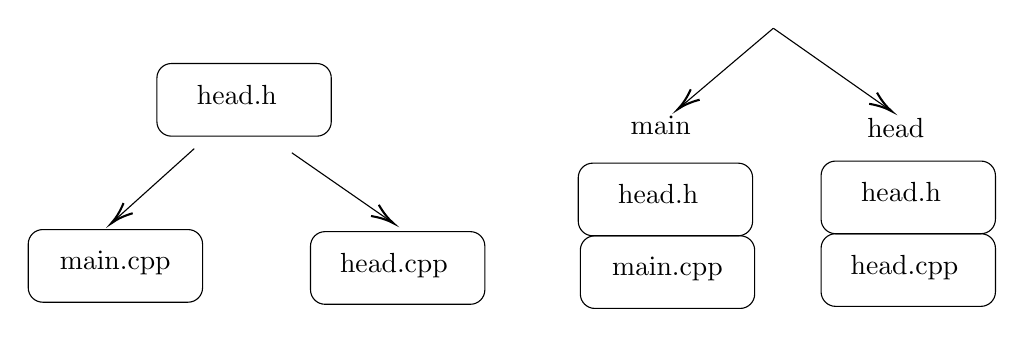
\begin{tikzpicture}[x=0.75pt,y=0.75pt,yscale=-1,xscale=1]
	%uncomment if require: \path (0,300); %set diagram left start at 0, and has height of 300
	
	%Rounded Rect [id:dp8046212658933671] 
	\draw   (119,83) .. controls (119,79.13) and (122.13,76) .. (126,76) -- (196,76) .. controls (199.87,76) and (203,79.13) .. (203,83) -- (203,104) .. controls (203,107.87) and (199.87,111) .. (196,111) -- (126,111) .. controls (122.13,111) and (119,107.87) .. (119,104) -- cycle ;
	%Rounded Rect [id:dp4131717476038639] 
	\draw   (57,163) .. controls (57,159.13) and (60.13,156) .. (64,156) -- (134,156) .. controls (137.87,156) and (141,159.13) .. (141,163) -- (141,184) .. controls (141,187.87) and (137.87,191) .. (134,191) -- (64,191) .. controls (60.13,191) and (57,187.87) .. (57,184) -- cycle ;
	%Rounded Rect [id:dp6275602235598181] 
	\draw   (193,164) .. controls (193,160.13) and (196.13,157) .. (200,157) -- (270,157) .. controls (273.87,157) and (277,160.13) .. (277,164) -- (277,185) .. controls (277,188.87) and (273.87,192) .. (270,192) -- (200,192) .. controls (196.13,192) and (193,188.87) .. (193,185) -- cycle ;
	%Straight Lines [id:da29892507643017163] 
	\draw    (137,117) -- (98.49,151.66) ;
	\draw [shift={(97,153)}, rotate = 318.01] [color={rgb, 255:red, 0; green, 0; blue, 0 }  ][line width=0.75]    (10.93,-3.29) .. controls (6.95,-1.4) and (3.31,-0.3) .. (0,0) .. controls (3.31,0.3) and (6.95,1.4) .. (10.93,3.29)   ;
	%Straight Lines [id:da7604434249637251] 
	\draw    (184,119) -- (231.36,151.86) ;
	\draw [shift={(233,153)}, rotate = 214.76] [color={rgb, 255:red, 0; green, 0; blue, 0 }  ][line width=0.75]    (10.93,-3.29) .. controls (6.95,-1.4) and (3.31,-0.3) .. (0,0) .. controls (3.31,0.3) and (6.95,1.4) .. (10.93,3.29)   ;
	%Rounded Rect [id:dp8118464469584348] 
	\draw   (439,165) .. controls (439,161.13) and (442.13,158) .. (446,158) -- (516,158) .. controls (519.87,158) and (523,161.13) .. (523,165) -- (523,186) .. controls (523,189.87) and (519.87,193) .. (516,193) -- (446,193) .. controls (442.13,193) and (439,189.87) .. (439,186) -- cycle ;
	%Rounded Rect [id:dp6893102005714937] 
	\draw   (323,166) .. controls (323,162.13) and (326.13,159) .. (330,159) -- (400,159) .. controls (403.87,159) and (407,162.13) .. (407,166) -- (407,187) .. controls (407,190.87) and (403.87,194) .. (400,194) -- (330,194) .. controls (326.13,194) and (323,190.87) .. (323,187) -- cycle ;
	%Rounded Rect [id:dp2970948370150095] 
	\draw   (322,131) .. controls (322,127.13) and (325.13,124) .. (329,124) -- (399,124) .. controls (402.87,124) and (406,127.13) .. (406,131) -- (406,152) .. controls (406,155.87) and (402.87,159) .. (399,159) -- (329,159) .. controls (325.13,159) and (322,155.87) .. (322,152) -- cycle ;
	%Rounded Rect [id:dp3048285006841027] 
	\draw   (439,130) .. controls (439,126.13) and (442.13,123) .. (446,123) -- (516,123) .. controls (519.87,123) and (523,126.13) .. (523,130) -- (523,151) .. controls (523,154.87) and (519.87,158) .. (516,158) -- (446,158) .. controls (442.13,158) and (439,154.87) .. (439,151) -- cycle ;
	%Straight Lines [id:da8496668043021236] 
	\draw    (416,59) -- (371.53,96.71) ;
	\draw [shift={(370,98)}, rotate = 319.71] [color={rgb, 255:red, 0; green, 0; blue, 0 }  ][line width=0.75]    (10.93,-3.29) .. controls (6.95,-1.4) and (3.31,-0.3) .. (0,0) .. controls (3.31,0.3) and (6.95,1.4) .. (10.93,3.29)   ;
	%Straight Lines [id:da057864555520047656] 
	\draw    (416,59) -- (471.36,97.85) ;
	\draw [shift={(473,99)}, rotate = 215.06] [color={rgb, 255:red, 0; green, 0; blue, 0 }  ][line width=0.75]    (10.93,-3.29) .. controls (6.95,-1.4) and (3.31,-0.3) .. (0,0) .. controls (3.31,0.3) and (6.95,1.4) .. (10.93,3.29)   ;
	
	% Text Node
	\draw (137,85) node [anchor=north west][inner sep=0.75pt]   [align=left] {head.h};
	% Text Node
	\draw (71,165) node [anchor=north west][inner sep=0.75pt]   [align=left] {main.cpp};
	% Text Node
	\draw (206,166) node [anchor=north west][inner sep=0.75pt]   [align=left] {head.cpp};
	% Text Node
	\draw (452,167) node [anchor=north west][inner sep=0.75pt]   [align=left] {head.cpp};
	% Text Node
	\draw (337,168) node [anchor=north west][inner sep=0.75pt]   [align=left] {main.cpp};
	% Text Node
	\draw (340,133) node [anchor=north west][inner sep=0.75pt]   [align=left] {head.h};
	% Text Node
	\draw (457,132) node [anchor=north west][inner sep=0.75pt]   [align=left] {head.h};
	% Text Node
	\draw (346,100) node [anchor=north west][inner sep=0.75pt]   [align=left] {main};
	% Text Node
	\draw (460,101) node [anchor=north west][inner sep=0.75pt]   [align=left] {head};
	
	
	\end{tikzpicture}
\end{center}

\noindent 每个翻译单元由编译器单独编译, 最终将得到的.o文件链接得到可执行文件. 如上图所示程序结构, 在链接时会出现如下问题:

假如在{\tt head.h}文件中定义一个外部链接性变量

\begin{lstlisting}[xleftmargin=2em]
#ifndef HEAD_H
#define HEAD_H
int i = 0;
#endif
\end{lstlisting}
那么在链接时就会出错, 原因是如上两个翻译单元相当于

\begin{center}
	\tikzset{every picture/.style={line width=0.75pt}} %set default line width to 0.75pt        
	
	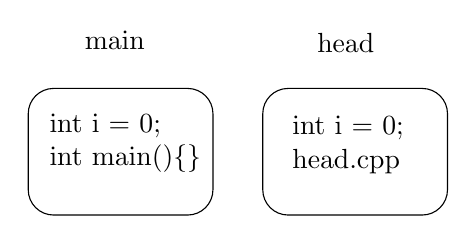
\begin{tikzpicture}[x=0.75pt,y=0.75pt,yscale=-1,xscale=1]
	%uncomment if require: \path (0,300); %set diagram left start at 0, and has height of 300
	
	%Rounded Rect [id:dp31960853174211556] 
	\draw   (225,159.2) .. controls (225,152.46) and (230.46,147) .. (237.2,147) -- (301.8,147) .. controls (308.54,147) and (314,152.46) .. (314,159.2) -- (314,195.8) .. controls (314,202.54) and (308.54,208) .. (301.8,208) -- (237.2,208) .. controls (230.46,208) and (225,202.54) .. (225,195.8) -- cycle ;
	%Rounded Rect [id:dp47295061263468985] 
	\draw   (338,159.2) .. controls (338,152.46) and (343.46,147) .. (350.2,147) -- (414.8,147) .. controls (421.54,147) and (427,152.46) .. (427,159.2) -- (427,195.8) .. controls (427,202.54) and (421.54,208) .. (414.8,208) -- (350.2,208) .. controls (343.46,208) and (338,202.54) .. (338,195.8) -- cycle ;
	
	% Text Node
	\draw (251,118) node [anchor=north west][inner sep=0.75pt]   [align=left] {main};
	% Text Node
	\draw (363,119) node [anchor=north west][inner sep=0.75pt]   [align=left] {head};
	% Text Node
	\draw (234,158) node [anchor=north west][inner sep=0.75pt]   [align=left] {int i = 0;\\int main()\{\}};
	% Text Node
	\draw (351,159.2) node [anchor=north west][inner sep=0.75pt]   [align=left] {int i = 0;\\head.cpp};
	
	
	\end{tikzpicture}
\end{center}

在两个文件中都定义了具有外部链接性的变量i.

在一个作用域内, 变量能且只能被定义一次, 但是可以被多次声明({\tt one define rule})
\begin{paracol}{2}
	\begin{leftcolumn}
		\begin{lstlisting}[title=定义,xleftmargin=2em,xrightmargin=2em]
// 不能在局部作用域内使用
extern int v = 0; 
int v;
		\end{lstlisting}
	\end{leftcolumn}
	\begin{rightcolumn}
		\begin{lstlisting}[title=声明,xleftmargin=2em,xrightmargin=2em]
void func();
extern void func();
extern int v;
		\end{lstlisting}
	\end{rightcolumn}
\end{paracol}

如果需要在多个文件, 指个多翻译单元中使用同一变量, 就必须把定义与声明分离. 变量的定义只能出现在一个文件中, 而在其它用到该变量
	的文件中对其声明.

所以往往头文件中只放一些声明而在另外的文件中进行定义.

\begin{paracol}{2}
	\begin{leftcolumn}
		常见的内部链接类型
		\begin{enumerate}
			\item {\tt const}全局变量
			\item {\tt static}全局变量
			\item {\tt static}函数
			\item {\tt inline}\footnote[1]{{\tt inline} 现在表示在链接时遇到不同编译单元出现了相同签名的函数时只保留一份, 不在是內联的意思.}函数/变量\footnote[2]{{\tt inline variable is C++17 extension}}
			\item 类内定义的成员函数
			\item 类内定义的数据成员(即非静态数据成员)
		\end{enumerate}
	\end{leftcolumn}
	\begin{rightcolumn}
		常见的外部链接类型
		\begin{enumerate}
			\item 全局变量与函数(非{\tt const、static、inline})
			\item 类外定义的数据成员(即静态数据成员在类外的定义)
			\item 类外定义的成员函数
			\item {\tt extern const T v = INIT;}
		\end{enumerate}
	\end{rightcolumn}
\end{paracol}
其它可视为无链接

\vspace{1em}
所有文件中的外部链接性变量会传递给链接器得到一张导出符号表. 记录本编译单元定义, 并且可提供给其它单元
	使用的符号及在本单元对应的地址. 

所有文件中的声明会传递给链接器得到一张未解决符号表, 记录本编译单元有声明但不在本单元定义的符号及其对应的地址, 
	显然在导出符号表中不能存在相同的符号.

\noindent{\tt C11}标准关于{\tt static}和{\tt extern}的内容:
\begin{enumerate}
	\item 若在{\tt extern}声明标识符之前的可见范围内存在对该标识符的声明, 则该标识符的链接与先前声明相同. 
			若无先前声明, 或声明无链接, 则该标识符具有外部链接
	\item 如果在同一翻译单元内, 同一标识符同时出现内外部链接, 则行为未定义
\end{enumerate}
上述原文:

{\tt For an identifier declared with the storage-class specifier extern in a scope 
in which a prior declaration of that identifier is visible, if the prior 
declaration specifies internal or external linkage, the linkage of the 
identifier at the later declaration is the same as the linkage specified 
at the prior declaration. If no prior declaration is visible, or if the 
prior declaration specifies no linkage, then the identifier has external 
linkage.

If, within a translation unit, the same identifier appears with both internal 
and external linkage, the behavior is undefined.}
\subsection{<===>\color{purple}{指针与引用}}
\subsubsection{指针与引用的区别}
\begin{enumerate}
	\item 引用就是常量指针
	\item 引用必须初始化, 且不能改变指向
	\item 无法对引用进行取地址, 或者说只能取到引用指向的对象的地址
	\item 引用的解引用操作由编译器自动进行
\end{enumerate}
\subsubsection{\tt{void*}指针}
指针一般有三个含义
\begin{enumerate}
	\item 指明数据的位置, 体现在指针的值
	\item 表示数据的大小, 例如{\tt int}指针表示四个字节为一组的数据, 体现在指针的步长、自身的加减法计算
	\item 表示数据如何被解释, 例如{\tt float}和{\tt int}都是四字节, 但解释结果完全不同, 体现在指针解引用的结果
\end{enumerate}

{\tt void*} 指针为第一种, 只指明了数据的位置. 以{\tt void*}的视角来看内存空间也仅仅是内存空间, 没办法访问内存空间中所存的对象

对于{\tt void*}类型指针与其它类型指针的转换, {\tt C++}有如下两个规定
\begin{enumerate}
	\item 不允许从{\tt void*}类型到其它类型的隐式转换, 允许从其它类型到{\tt void*}类型的隐式转换, 常见于函数传参
	\item 字面量0可以隐式转换成任意类型的空指针常量
\end{enumerate}

\subsubsection{\tt{nullptr\quad <11>}}

在{\tt C}中, 常用{\tt NULL}来表示空指针
\begin{lstlisting}[xleftmargin=2em]
#define NULL ((void*)0)
\end{lstlisting}
然而在{\tt C++}中不允许从{\tt void*}隐式转换成其它类型的指针, 所以定义了一种新的指针类型, 指针空值类型{\tt std::nullptr\_t}
	, {\tt nullptr}是它的一个实例, 当对指针进行初始化时:
\begin{lstlisting}[xleftmargin=2em]
int *p = nullptr;
int *p = 0;
\end{lstlisting}
两者之间没有区别

\noindent 但在重载情况下:
\begin{lstlisting}[xleftmargin=2em]
void func(int n);
void func(int *p);
\end{lstlisting}
{\tt nullptr}会匹配第二个, 而0实际上两个都能匹配, 在本实验环境中, 会匹配第一项且没有二义性问题

\noindent 若再定义一个
\begin{lstlisting}[xleftmargin=2em]
void func(char *p);
\end{lstlisting}
则{\tt nullptr}会出现二义性错误

至于空指针具体指向哪个地址由编译器管理, 可能是内存中的0号地址, 即指针数据全是0, 也有可能不是

%Effective Modern C++ 第8款, 使用nullptr 而非0, NULL.\\

\subsubsection{野指针}

{\tt wild pointer}也叫悬挂指针, {\tt dangling pointer}

有三种情况会造成野指针:
\begin{enumerate}
	\item 指针未初始化
	\item 指针指向的对象生命周期结束, 如将一个函数体内的局部变量地址传递给外部指针
	\item 指针释放
\end{enumerate}

当指针被{\tt delete}之后, 指针值变为无效, 继续对该指针进行操作会出现{\tt heap use after free}错误.

事实上, 当一个指针被{\tt delete}之后, 指针指向的堆地址空间被释放, 随时可以被分配给其它对象, 但在不同的机器上会有不同的结果.

\noindent 几种特殊情况, 指{\tt delete}之后继续使用指针不报错的情况:
\begin{enumerate}
	\item 指针的数据, 即它指向的地址发生改变, 对它进行解引用会得到0
	\item 地址不改变, 解引用会得到0
	\item 地址不改变, 该内存地址的值也未被擦除, 解引用得到跟{\tt delete}之前一样的结果
\end{enumerate}

准确来讲, {\tt delete}的实际意义是将指针指向的内存空间释放, 以便能分配给其它对象, 但指针本身是否依旧指向那块内存, 
	那块内存的数据是否被擦除未定义

给野指针赋{\tt nullptr}初值避免麻烦

\subsubsection{指向引用的指针, 指向指针的引用}
对引用地址的获取行为会得到引用指向的对象的地址

测试程序见 \href{https://github.com/wenqingqian/Obtuse/blob/main/test/cpp/basic/pointer_reference.cpp}{\tt pointer\_reference}

\begin{center}


	\tikzset{every picture/.style={line width=0.75pt}} %set default line width to 0.75pt        

	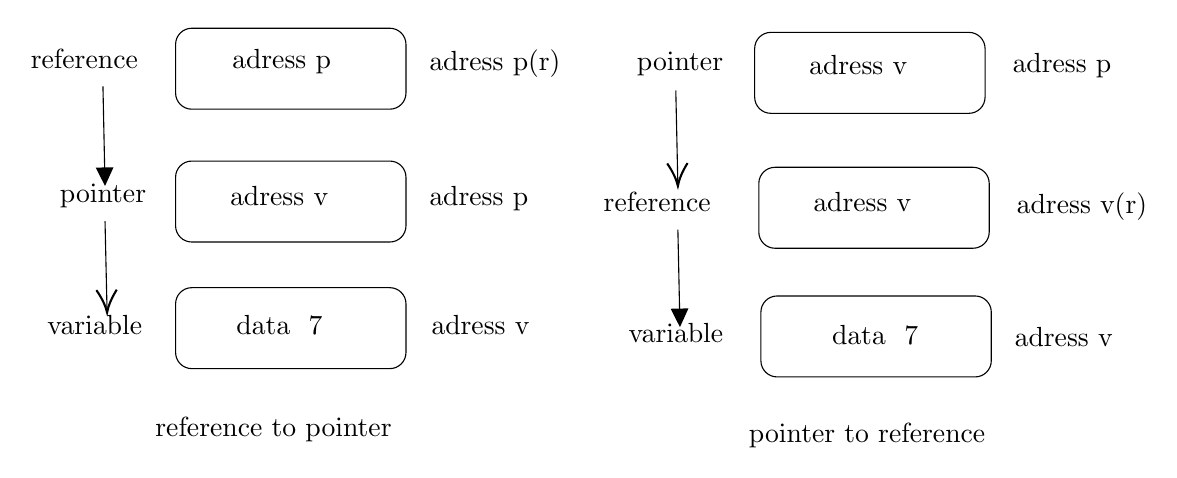
\begin{tikzpicture}[x=0.75pt,y=0.75pt,yscale=-1,xscale=1]
	%uncomment if require: \path (0,300); %set diagram left start at 0, and has height of 300
	
	%Rounded Rect [id:dp11927883071932444] 
	\draw   (85,185.8) .. controls (85,181.49) and (88.49,178) .. (92.8,178) -- (188.2,178) .. controls (192.51,178) and (196,181.49) .. (196,185.8) -- (196,209.2) .. controls (196,213.51) and (192.51,217) .. (188.2,217) -- (92.8,217) .. controls (88.49,217) and (85,213.51) .. (85,209.2) -- cycle ;
	%Rounded Rect [id:dp6640212087116251] 
	\draw   (85,124.8) .. controls (85,120.49) and (88.49,117) .. (92.8,117) -- (188.2,117) .. controls (192.51,117) and (196,120.49) .. (196,124.8) -- (196,148.2) .. controls (196,152.51) and (192.51,156) .. (188.2,156) -- (92.8,156) .. controls (88.49,156) and (85,152.51) .. (85,148.2) -- cycle ;
	%Rounded Rect [id:dp3237041947663375] 
	\draw   (85,60.8) .. controls (85,56.49) and (88.49,53) .. (92.8,53) -- (188.2,53) .. controls (192.51,53) and (196,56.49) .. (196,60.8) -- (196,84.2) .. controls (196,88.51) and (192.51,92) .. (188.2,92) -- (92.8,92) .. controls (88.49,92) and (85,88.51) .. (85,84.2) -- cycle ;
	%Rounded Rect [id:dp9477857736296029] 
	\draw   (367,189.8) .. controls (367,185.49) and (370.49,182) .. (374.8,182) -- (470.2,182) .. controls (474.51,182) and (478,185.49) .. (478,189.8) -- (478,213.2) .. controls (478,217.51) and (474.51,221) .. (470.2,221) -- (374.8,221) .. controls (370.49,221) and (367,217.51) .. (367,213.2) -- cycle ;
	%Rounded Rect [id:dp4721875816932608] 
	\draw   (366,127.8) .. controls (366,123.49) and (369.49,120) .. (373.8,120) -- (469.2,120) .. controls (473.51,120) and (477,123.49) .. (477,127.8) -- (477,151.2) .. controls (477,155.51) and (473.51,159) .. (469.2,159) -- (373.8,159) .. controls (369.49,159) and (366,155.51) .. (366,151.2) -- cycle ;
	%Rounded Rect [id:dp34593900558257906] 
	\draw   (364,62.8) .. controls (364,58.49) and (367.49,55) .. (371.8,55) -- (467.2,55) .. controls (471.51,55) and (475,58.49) .. (475,62.8) -- (475,86.2) .. controls (475,90.51) and (471.51,94) .. (467.2,94) -- (371.8,94) .. controls (367.49,94) and (364,90.51) .. (364,86.2) -- cycle ;
	%Straight Lines [id:da5154723980908134] 
	\draw    (51,146) -- (51.95,188) ;
	\draw [shift={(52,190)}, rotate = 268.7] [color={rgb, 255:red, 0; green, 0; blue, 0 }  ][line width=0.75]    (10.93,-4.9) .. controls (6.95,-2.3) and (3.31,-0.67) .. (0,0) .. controls (3.31,0.67) and (6.95,2.3) .. (10.93,4.9)   ;
	%Straight Lines [id:da5246033953497637] 
	\draw    (50,81) -- (50.94,126) ;
	\draw [shift={(51,129)}, rotate = 268.81] [fill={rgb, 255:red, 0; green, 0; blue, 0 }  ][line width=0.08]  [draw opacity=0] (8.93,-4.29) -- (0,0) -- (8.93,4.29) -- cycle    ;
	%Straight Lines [id:da36423552536908654] 
	\draw    (327,150) -- (327.94,194) ;
	\draw [shift={(328,197)}, rotate = 268.78] [fill={rgb, 255:red, 0; green, 0; blue, 0 }  ][line width=0.08]  [draw opacity=0] (8.93,-4.29) -- (0,0) -- (8.93,4.29) -- cycle    ;
	%Straight Lines [id:da2981001586744325] 
	\draw    (326,83) -- (326.96,127) ;
	\draw [shift={(327,129)}, rotate = 268.75] [color={rgb, 255:red, 0; green, 0; blue, 0 }  ][line width=0.75]    (10.93,-4.9) .. controls (6.95,-2.3) and (3.31,-0.67) .. (0,0) .. controls (3.31,0.67) and (6.95,2.3) .. (10.93,4.9)   ;
	
	% Text Node
	\draw (74,239) node [anchor=north west][inner sep=0.75pt]   [align=left] {reference to pointer};
	% Text Node
	\draw (360,242) node [anchor=north west][inner sep=0.75pt]   [align=left] {pointer to reference};
	% Text Node
	\draw (113,190) node [anchor=north west][inner sep=0.75pt]   [align=left] {data \ 7};
	% Text Node
	\draw (22,190) node [anchor=north west][inner sep=0.75pt]   [align=left] {variable};
	% Text Node
	\draw (207,190) node [anchor=north west][inner sep=0.75pt]   [align=left] {adress v};
	% Text Node
	\draw (28,127) node [anchor=north west][inner sep=0.75pt]   [align=left] {pointer};
	% Text Node
	\draw (206,128) node [anchor=north west][inner sep=0.75pt]   [align=left] {adress p};
	% Text Node
	\draw (14,62) node [anchor=north west][inner sep=0.75pt]   [align=left] {reference};
	% Text Node
	\draw (206,62) node [anchor=north west][inner sep=0.75pt]   [align=left] {adress p(r)};
	% Text Node
	\draw (111,62) node [anchor=north west][inner sep=0.75pt]   [align=left] {adress p};
	% Text Node
	\draw (110,128) node [anchor=north west][inner sep=0.75pt]   [align=left] {adress v};
	% Text Node
	\draw (290,131) node [anchor=north west][inner sep=0.75pt]   [align=left] {reference};
	% Text Node
	\draw (306,63) node [anchor=north west][inner sep=0.75pt]   [align=left] {pointer};
	% Text Node
	\draw (302,194) node [anchor=north west][inner sep=0.75pt]   [align=left] {variable};
	% Text Node
	\draw (488,196) node [anchor=north west][inner sep=0.75pt]   [align=left] {adress v};
	% Text Node
	\draw (400,195) node [anchor=north west][inner sep=0.75pt]   [align=left] {data \ 7};
	% Text Node
	\draw (487,64) node [anchor=north west][inner sep=0.75pt]   [align=left] {adress p};
	% Text Node
	\draw (489,131) node [anchor=north west][inner sep=0.75pt]   [align=left] {adress v(r)};
	% Text Node
	\draw (391,131) node [anchor=north west][inner sep=0.75pt]   [align=left] {adress v};
	% Text Node
	\draw (389,65) node [anchor=north west][inner sep=0.75pt]   [align=left] {adress v};
	
	
	\end{tikzpicture}
\end{center}
\subsection{\color{purple}{{\tt const}关键字}}
\subsection{\color{purple}{{\tt malloc}和{\tt new}区别}}
%------------------------------------------------------------------------------------------------%
%-------------------------------------Section object-oriented---------------------------%
%------------------------------------------------------------------------------------------------%
\section{\color{blue}{面向对象}}

\subsection[多态的实现原理和应用场景]{\color{purple}{多态的实现原理和应用场景}}
%------------------------------------------------------------------------------------------------%
%-------------------------------------Section STL---------------------------------------%
%------------------------------------------------------------------------------------------------%
\section{\color{blue}{\tt STL}}

\subsection{\color{purple}{线程安全的实现及标准容器库的线程安全性}}
\subsection{\color{purple}{{\tt sort}算法是怎么实现的}}

%------------------------------------------------------------------------------------------------%
%-------------------------------------Section C++11------------------------------------%
\section{\color{blue}{\tt C++11}}

\subsection{<===>\color{purple}{\tt{decltype}和\tt{auto}}}

\columnratio{0.5}
\begin{paracol}{2}
	\begin{leftcolumn}
		\begin{lstlisting}[title=decltype,basicstyle=\small,columns=flexible,xleftmargin=2em,xrightmargin=2em]
int *r=0;
decltype (*r+0) a;//表达式结果为int, 因此a为int
decltype (r) a;//a是指针
decltype (*r) a = ini;//a是引用
decltype ((r)) a = ini;//a是指向指针的引用
decltype ((*r)) a = ini;//a是引用 
		\end{lstlisting}
		{\tt decltype((variable))}的结果永远是引用.
	\end{leftcolumn}
	\begin{rightcolumn}
		\uline{{\tt auto}一般会忽略顶层{\tt const}, 保留底层{\tt const}}, 引用本身就是一个顶层{\tt const}指针, 因此{\tt auto}类型推导不会直接得到引用类型
		\begin{lstlisting}[basicstyle=\small,columns=flexible,xleftmargin=2em,xrightmargin=2em]
const int i = 1; const int&r = i;
auto a = i;//a是int
auto a = &i;//a是const int*(底层const)
auto a = r;//a是int
auto &a = i;//a是左引用
auto &&a;(万能引用)
		\end{lstlisting}
	\end{rightcolumn}
\end{paracol}
\subsection{<===>\color{purple}{左右值}}
\subsubsection{左值与右值}
 \href{https://zhuanlan.zhihu.com/p/402251966}{原文}

左值是一个对象, 可以用\&取地址, 而右值更贴近“值”本身. 一般来说, 表达式结束后, 
	值是否有\uline{显式}的存储位置是左右值的区分(右值可以隐式存在内存中)

\columnratio{0.5}
\begin{paracol}{2}
	\begin{leftcolumn}
		左值:
		\begin{enumerate}
			\item 字符串字面量
			\item 内置的前{\tt ++}与前{\tt --}
			\item 右值引用类型变量
			\item 转型为左值引用的表达式
			\item *解引用的表达式
		\end{enumerate}
	\end{leftcolumn}
	\begin{rightcolumn}
		右值:
		\begin{enumerate}
			\item 非字符串的字面量以及枚举项
			\item 置的后{\tt++}与后{\tt- -}
			\item 内置的算术, 逻辑, 比较表达式
			\item 内置取地址表达式, {\tt this}指针
			\item 未命名的{\tt lambda}表达式
			\item 转型为非引用的表达式
			\item 转型为右值引用的表达式
		\end{enumerate}
	\end{rightcolumn}
\end{paracol}
\subsubsection{左值引用与右值引用}

左右值并不是{\tt C++11}才有的新概念, 而右值引用是{\tt C++11}为了处理
	无需深拷贝的资源转移型需求而引入

左右引用只能处理对应的左右值. 一个例外是{\tt const T\&}, 既可以引用左值, 也可以引用右值

\noindent 即可以写出这样的代码
\begin{lstlisting}[basicstyle=\small,columns=flexible,xleftmargin=16em,xrightmargin=16em]
const int& clr = 1; const int& clr2 = clr;
\end{lstlisting}

\vspace*{2em}
\columnratio{0.4}
\begin{paracol}{2}
	\begin{leftcolumn}
		对于右值来说, 不能真正取地址, 而引用实质就是操作地址指针, 因此理论上无法进行左引用. 对于左值来说, 
			可以显式转换成右值引用

		如右值例7, 转换为右值引用的表达式本身是一个右值, 但是通过右值引用绑定到的对象自身是一个左值, 即左值例3
	\end{leftcolumn}
	\begin{rightcolumn}
		\begin{lstlisting}[basicstyle=\small,columns=flexible,xleftmargin=5em,xrightmargin=5em]
//可以将左值转为右值, 再进行右引用
Test t(1);
// 使用std::move转为右值引用
Test&& t1 = std::move(t);
// 使用static_cast转为右值引用
Test&& t2 = static_cast<Test&&>(t);
// 使用C风格强转为右值引用
Test&& t3 = (Test&&)t;
// 使用std::forwad<T&&>为右值引用
Test&& t4 = std::forward<T&&>(t);
		\end{lstlisting}
	\end{rightcolumn}
\end{paracol}
\subsection{<===>\color{purple}{移动语义与完美转发}}
\subsubsection{浅拷贝与深拷贝}
\columnratio{0.5}
\begin{paracol}{2}
	
	\begin{leftcolumn}
	当通过一个对象初始化另一个对象时,

	如 \uline{{\tt Test a(10);}}\uline{{\tt Test b(a);}}时:

	假设{\tt Test}中有资源拖管
		
	只记录资源{\tt Data}的指针, 而非记录资源全部信息到类对象里面, 
		构造时从堆上用{\tt new}申请内存供资源后面使用, 析构时从堆上释放内存, 回收掉资源, 
		中间过程资源读写操作都通过指针{\tt p}来完成. {\tt C++}对象构造与析构函数的成对调用, 
		也保证了安全性与不发生泄露({\tt RAII})
	\end{leftcolumn}
	\begin{rightcolumn}
\begin{lstlisting}[xleftmargin=2em,xrightmargin=2em]
class Test1 public:
	Test1(int s):size(s) 
		p = new char[size];
	~Test1()
		if(p)  delete []p; 
			   p = nullptr;
	int size;
	char* p;
\end{lstlisting}	
	\end{rightcolumn}
\end{paracol}

以右侧结构为例: 

\begin{center}




	\tikzset{every picture/.style={line width=0.75pt}} %set default line width to 0.75pt        

	\begin{tikzpicture}[x=0.75pt,y=0.75pt,yscale=-1,xscale=1]
	%uncomment if require: \path (0,246); %set diagram left start at 0, and has height of 246
	
	%Rounded Rect [id:dp9814564185052337] 
	\draw   (144.09,96.49) .. controls (144.09,92.04) and (147.7,88.43) .. (152.15,88.43) -- (198.94,88.43) .. controls (203.39,88.43) and (207,92.04) .. (207,96.49) -- (207,120.68) .. controls (207,125.13) and (203.39,128.74) .. (198.94,128.74) -- (152.15,128.74) .. controls (147.7,128.74) and (144.09,125.13) .. (144.09,120.68) -- cycle ;
	%Rounded Rect [id:dp13504310460610203] 
	\draw   (3,96.49) .. controls (3,92.04) and (6.61,88.43) .. (11.06,88.43) -- (57.85,88.43) .. controls (62.3,88.43) and (65.91,92.04) .. (65.91,96.49) -- (65.91,120.68) .. controls (65.91,125.13) and (62.3,128.74) .. (57.85,128.74) -- (11.06,128.74) .. controls (6.61,128.74) and (3,125.13) .. (3,120.68) -- cycle ;
	%Shape: Ellipse [id:dp35837246392687105] 
	\draw   (11.99,170.01) .. controls (11.99,156.76) and (22.05,146.01) .. (34.45,146.01) .. controls (46.86,146.01) and (56.92,156.76) .. (56.92,170.01) .. controls (56.92,183.26) and (46.86,194) .. (34.45,194) .. controls (22.05,194) and (11.99,183.26) .. (11.99,170.01) -- cycle ;
	%Rounded Rect [id:dp20403462657508187] 
	\draw   (362.7,96.38) .. controls (362.7,91.97) and (366.28,88.39) .. (370.69,88.39) -- (421.01,88.39) .. controls (425.42,88.39) and (429,91.97) .. (429,96.38) -- (429,120.34) .. controls (429,124.75) and (425.42,128.33) .. (421.01,128.33) -- (370.69,128.33) .. controls (366.28,128.33) and (362.7,124.75) .. (362.7,120.34) -- cycle ;
	%Rounded Rect [id:dp7768537420240913] 
	\draw   (214,96.38) .. controls (214,91.97) and (217.58,88.39) .. (221.99,88.39) -- (272.31,88.39) .. controls (276.72,88.39) and (280.3,91.97) .. (280.3,96.38) -- (280.3,120.34) .. controls (280.3,124.75) and (276.72,128.33) .. (272.31,128.33) -- (221.99,128.33) .. controls (217.58,128.33) and (214,124.75) .. (214,120.34) -- cycle ;
	%Shape: Ellipse [id:dp5039225164311434] 
	\draw   (220.47,171.22) .. controls (220.47,158.09) and (231.07,147.45) .. (244.15,147.45) .. controls (257.23,147.45) and (267.83,158.09) .. (267.83,171.22) .. controls (267.83,184.36) and (257.23,195) .. (244.15,195) .. controls (231.07,195) and (220.47,184.36) .. (220.47,171.22) -- cycle ;
	%Shape: Ellipse [id:dp3337480641475472] 
	\draw   (371.17,170.32) .. controls (371.17,157.19) and (381.77,146.55) .. (394.85,146.55) .. controls (407.93,146.55) and (418.53,157.19) .. (418.53,170.32) .. controls (418.53,183.45) and (407.93,194.1) .. (394.85,194.1) .. controls (381.77,194.1) and (371.17,183.45) .. (371.17,170.32) -- cycle ;
	%Rounded Rect [id:dp44340954001106425] 
	\draw   (585.39,96.85) .. controls (585.39,92.61) and (588.83,89.17) .. (593.07,89.17) -- (644.32,89.17) .. controls (648.56,89.17) and (652,92.61) .. (652,96.85) -- (652,119.89) .. controls (652,124.13) and (648.56,127.57) .. (644.32,127.57) -- (593.07,127.57) .. controls (588.83,127.57) and (585.39,124.13) .. (585.39,119.89) -- cycle ;
	%Rounded Rect [id:dp7095396196135548] 
	\draw   (436,96.85) .. controls (436,92.61) and (439.44,89.17) .. (443.68,89.17) -- (494.93,89.17) .. controls (499.17,89.17) and (502.61,92.61) .. (502.61,96.85) -- (502.61,119.89) .. controls (502.61,124.13) and (499.17,127.57) .. (494.93,127.57) -- (443.68,127.57) .. controls (439.44,127.57) and (436,124.13) .. (436,119.89) -- cycle ;
	%Shape: Ellipse [id:dp8281848505805895] 
	\draw   (504.52,167.88) .. controls (504.52,155.25) and (515.17,145.02) .. (528.3,145.02) .. controls (541.44,145.02) and (552.09,155.25) .. (552.09,167.88) .. controls (552.09,180.5) and (541.44,190.73) .. (528.3,190.73) .. controls (515.17,190.73) and (504.52,180.5) .. (504.52,167.88) -- cycle ;
	\draw   (492.61,127.03) -- (489.54,146.53)(500.9,138.32) -- (481.25,135.24) ;
	
	% Text Node
	\draw (84.56,18.13) node [anchor=north west][inner sep=0.75pt]  [font=\normalsize] [align=left] {浅拷贝};
	% Text Node
	\draw (304.76,12.92) node [anchor=north west][inner sep=0.75pt]  [font=\normalsize] [align=left] {深拷贝};
	% Text Node
	\draw (23.56,53.58) node [anchor=north west][inner sep=0.75pt]  [font=\small] [align=left] {old};
	% Text Node
	\draw (161.6,52.62) node [anchor=north west][inner sep=0.75pt]  [font=\small] [align=left] {new};
	% Text Node
	\draw (94.55,48.55) node [anchor=north west][inner sep=0.75pt]  [font=\small,rotate=-359.26] [align=left] {copy};
	% Text Node
	\draw (151.21,91.01) node [anchor=north west][inner sep=0.75pt]  [font=\small] [align=left] {int size};
	% Text Node
	\draw (152.6,109.24) node [anchor=north west][inner sep=0.75pt]  [font=\small] [align=left] {char* p};
	% Text Node
	\draw (10.12,91.01) node [anchor=north west][inner sep=0.75pt]  [font=\small] [align=left] {int size};
	% Text Node
	\draw (9.71,108.28) node [anchor=north west][inner sep=0.75pt]  [font=\small] [align=left] {char* p};
	% Text Node
	\draw (19.43,154.18) node [anchor=north west][inner sep=0.75pt]  [font=\small] [align=left] {new \\char[]};
	% Text Node
	\draw (94.39,84.91) node [anchor=north west][inner sep=0.75pt]  [font=\small,rotate=-359.26] [align=left] {copy};
	% Text Node
	\draw (95.45,103.14) node [anchor=north west][inner sep=0.75pt]  [font=\small,rotate=-359.26] [align=left] {copy};
	% Text Node
	\draw (236.2,53.79) node [anchor=north west][inner sep=0.75pt]  [font=\small] [align=left] {old};
	% Text Node
	\draw (381.88,52.83) node [anchor=north west][inner sep=0.75pt]  [font=\small] [align=left] {new};
	% Text Node
	\draw (311.27,48.8) node [anchor=north west][inner sep=0.75pt]  [font=\small,rotate=-359.26] [align=left] {copy};
	% Text Node
	\draw (371.39,90.87) node [anchor=north west][inner sep=0.75pt]  [font=\small] [align=left] {int size};
	% Text Node
	\draw (372.88,108.94) node [anchor=north west][inner sep=0.75pt]  [font=\small] [align=left] {char* p};
	% Text Node
	\draw (222.69,90.87) node [anchor=north west][inner sep=0.75pt]  [font=\small] [align=left] {int size};
	% Text Node
	\draw (222.28,107.99) node [anchor=north west][inner sep=0.75pt]  [font=\small] [align=left] {char* p};
	% Text Node
	\draw (230.15,156.42) node [anchor=north west][inner sep=0.75pt]  [font=\small] [align=left] {new \\char[]};
	% Text Node
	\draw (313.16,86.84) node [anchor=north west][inner sep=0.75pt]  [font=\small,rotate=-359.26] [align=left] {copy};
	% Text Node
	\draw (380.85,153.57) node [anchor=north west][inner sep=0.75pt]  [font=\small] [align=left] {new \\char[]};
	% Text Node
	\draw (313.16,149.61) node [anchor=north west][inner sep=0.75pt]  [font=\small,rotate=-359.26] [align=left] {copy};
	% Text Node
	\draw (523.28,11) node [anchor=north west][inner sep=0.75pt]  [font=\normalsize] [align=left] {移动语义};
	% Text Node
	\draw (458.35,55.62) node [anchor=north west][inner sep=0.75pt]  [font=\small] [align=left] {old};
	% Text Node
	\draw (604.72,54.71) node [anchor=north west][inner sep=0.75pt]  [font=\small] [align=left] {new};
	% Text Node
	\draw (533.78,50.87) node [anchor=north west][inner sep=0.75pt]  [font=\small,rotate=-359.26] [align=left] {move};
	% Text Node
	\draw (594.22,91.27) node [anchor=north west][inner sep=0.75pt]  [font=\small] [align=left] {int size};
	% Text Node
	\draw (595.72,108.64) node [anchor=north west][inner sep=0.75pt]  [font=\small] [align=left] {char* p};
	% Text Node
	\draw (444.83,91.27) node [anchor=north west][inner sep=0.75pt]  [font=\small] [align=left] {int size};
	% Text Node
	\draw (444.43,107.73) node [anchor=north west][inner sep=0.75pt]  [font=\small] [align=left] {char* p};
	% Text Node
	\draw (513.3,152.22) node [anchor=north west][inner sep=0.75pt]  [font=\small] [align=left] {new \\char[]};
	% Text Node
	\draw (535.69,87.44) node [anchor=north west][inner sep=0.75pt]  [font=\small,rotate=-359.26] [align=left] {copy};
	% Text Node
	\draw (537.69,102.44) node [anchor=north west][inner sep=0.75pt]  [font=\small,rotate=-359.26] [align=left] {copy};
	% Text Node
	\draw (450,166) node [anchor=north west][inner sep=0.75pt]  [font=\small] [align=left] {{\small nullptr}};
	% Connection
	\draw [color={rgb, 255:red, 175; green, 0; blue, 50 }  ,draw opacity=1 ]   (158.6,60.23) -- (48.56,60.98) ;
	\draw [shift={(46.56,60.99)}, rotate = 359.61] [color={rgb, 255:red, 175; green, 0; blue, 50 }  ,draw opacity=1 ][line width=0.75]    (10.93,-3.29) .. controls (6.95,-1.4) and (3.31,-0.3) .. (0,0) .. controls (3.31,0.3) and (6.95,1.4) .. (10.93,3.29)   ;
	% Connection
	\draw    (174.53,71.62) -- (173.87,85.01) ;
	\draw [shift={(173.78,87.01)}, rotate = 272.81] [color={rgb, 255:red, 0; green, 0; blue, 0 }  ][line width=0.75]    (10.93,-3.29) .. controls (6.95,-1.4) and (3.31,-0.3) .. (0,0) .. controls (3.31,0.3) and (6.95,1.4) .. (10.93,3.29)   ;
	% Connection
	\draw    (33.29,127.28) -- (35.26,148.19) ;
	\draw [shift={(35.45,150.18)}, rotate = 264.61] [color={rgb, 255:red, 0; green, 0; blue, 0 }  ][line width=0.75]    (10.93,-3.29) .. controls (6.95,-1.4) and (3.31,-0.3) .. (0,0) .. controls (3.31,0.3) and (6.95,1.4) .. (10.93,3.29)   ;
	% Connection
	\draw    (33.11,72.58) -- (32.64,85.01) ;
	\draw [shift={(32.56,87.01)}, rotate = 272.2] [color={rgb, 255:red, 0; green, 0; blue, 0 }  ][line width=0.75]    (10.93,-3.29) .. controls (6.95,-1.4) and (3.31,-0.3) .. (0,0) .. controls (3.31,0.3) and (6.95,1.4) .. (10.93,3.29)   ;
	% Connection
	\draw [color={rgb, 255:red, 175; green, 0; blue, 50 }  ,draw opacity=1 ]   (148.21,98.51) -- (59.12,98.51) ;
	\draw [shift={(57.12,98.51)}, rotate = 360] [color={rgb, 255:red, 175; green, 0; blue, 50 }  ,draw opacity=1 ][line width=0.75]    (10.93,-3.29) .. controls (6.95,-1.4) and (3.31,-0.3) .. (0,0) .. controls (3.31,0.3) and (6.95,1.4) .. (10.93,3.29)   ;
	% Connection
	\draw [color={rgb, 255:red, 175; green, 0; blue, 50 }  ,draw opacity=1 ]   (149.6,116.57) -- (59.71,115.97) ;
	\draw [shift={(57.71,115.95)}, rotate = 0.38] [color={rgb, 255:red, 175; green, 0; blue, 50 }  ,draw opacity=1 ][line width=0.75]    (10.93,-3.29) .. controls (6.95,-1.4) and (3.31,-0.3) .. (0,0) .. controls (3.31,0.3) and (6.95,1.4) .. (10.93,3.29)   ;
	% Connection
	\draw [color={rgb, 255:red, 175; green, 0; blue, 50 }  ,draw opacity=1 ]   (149.6,126.83) -- (60.29,162.14) ;
	\draw [shift={(58.43,162.88)}, rotate = 338.42] [color={rgb, 255:red, 175; green, 0; blue, 50 }  ,draw opacity=1 ][line width=0.75]    (10.93,-3.29) .. controls (6.95,-1.4) and (3.31,-0.3) .. (0,0) .. controls (3.31,0.3) and (6.95,1.4) .. (10.93,3.29)   ;
	% Connection
	\draw [color={rgb, 255:red, 175; green, 0; blue, 50 }  ,draw opacity=1 ]   (378.88,60.44) -- (261.2,61.19) ;
	\draw [shift={(259.2,61.2)}, rotate = 359.63] [color={rgb, 255:red, 175; green, 0; blue, 50 }  ,draw opacity=1 ][line width=0.75]    (10.93,-3.29) .. controls (6.95,-1.4) and (3.31,-0.3) .. (0,0) .. controls (3.31,0.3) and (6.95,1.4) .. (10.93,3.29)   ;
	% Connection
	\draw    (394.78,71.83) -- (394.09,84.88) ;
	\draw [shift={(393.99,86.87)}, rotate = 272.99] [color={rgb, 255:red, 0; green, 0; blue, 0 }  ][line width=0.75]    (10.93,-3.29) .. controls (6.95,-1.4) and (3.31,-0.3) .. (0,0) .. controls (3.31,0.3) and (6.95,1.4) .. (10.93,3.29)   ;
	% Connection
	\draw    (245.45,126.99) -- (246.81,150.42) ;
	\draw [shift={(246.93,152.42)}, rotate = 266.67] [color={rgb, 255:red, 0; green, 0; blue, 0 }  ][line width=0.75]    (10.93,-3.29) .. controls (6.95,-1.4) and (3.31,-0.3) .. (0,0) .. controls (3.31,0.3) and (6.95,1.4) .. (10.93,3.29)   ;
	% Connection
	\draw    (245.73,72.79) -- (245.24,84.88) ;
	\draw [shift={(245.16,86.87)}, rotate = 272.34] [color={rgb, 255:red, 0; green, 0; blue, 0 }  ][line width=0.75]    (10.93,-3.29) .. controls (6.95,-1.4) and (3.31,-0.3) .. (0,0) .. controls (3.31,0.3) and (6.95,1.4) .. (10.93,3.29)   ;
	% Connection
	\draw [color={rgb, 255:red, 175; green, 0; blue, 50 }  ,draw opacity=1 ]   (368.39,98.37) -- (271.69,98.37) ;
	\draw [shift={(269.69,98.37)}, rotate = 360] [color={rgb, 255:red, 175; green, 0; blue, 50 }  ,draw opacity=1 ][line width=0.75]    (10.93,-3.29) .. controls (6.95,-1.4) and (3.31,-0.3) .. (0,0) .. controls (3.31,0.3) and (6.95,1.4) .. (10.93,3.29)   ;
	% Connection
	\draw    (396.11,127.94) -- (397.37,147.57) ;
	\draw [shift={(397.5,149.57)}, rotate = 266.33] [color={rgb, 255:red, 0; green, 0; blue, 0 }  ][line width=0.75]    (10.93,-3.29) .. controls (6.95,-1.4) and (3.31,-0.3) .. (0,0) .. controls (3.31,0.3) and (6.95,1.4) .. (10.93,3.29)   ;
	% Connection
	\draw [color={rgb, 255:red, 175; green, 0; blue, 50 }  ,draw opacity=1 ]   (377.85,170.97) -- (271.15,172.99) ;
	\draw [shift={(269.15,173.02)}, rotate = 358.92] [color={rgb, 255:red, 175; green, 0; blue, 50 }  ,draw opacity=1 ][line width=0.75]    (10.93,-3.29) .. controls (6.95,-1.4) and (3.31,-0.3) .. (0,0) .. controls (3.31,0.3) and (6.95,1.4) .. (10.93,3.29)   ;
	% Connection
	\draw [color={rgb, 255:red, 175; green, 0; blue, 50 }  ,draw opacity=1 ]   (601.72,62.31) -- (483.35,63.03) ;
	\draw [shift={(481.35,63.04)}, rotate = 359.65] [color={rgb, 255:red, 175; green, 0; blue, 50 }  ,draw opacity=1 ][line width=0.75]    (10.93,-3.29) .. controls (6.95,-1.4) and (3.31,-0.3) .. (0,0) .. controls (3.31,0.3) and (6.95,1.4) .. (10.93,3.29)   ;
	% Connection
	\draw    (617.59,73.71) -- (616.96,85.28) ;
	\draw [shift={(616.85,87.27)}, rotate = 273.13] [color={rgb, 255:red, 0; green, 0; blue, 0 }  ][line width=0.75]    (10.93,-3.29) .. controls (6.95,-1.4) and (3.31,-0.3) .. (0,0) .. controls (3.31,0.3) and (6.95,1.4) .. (10.93,3.29)   ;
	% Connection
	\draw    (480.64,126.73) -- (508.77,150.32) ;
	\draw [shift={(510.3,151.61)}, rotate = 219.99] [color={rgb, 255:red, 0; green, 0; blue, 0 }  ][line width=0.75]    (10.93,-3.29) .. controls (6.95,-1.4) and (3.31,-0.3) .. (0,0) .. controls (3.31,0.3) and (6.95,1.4) .. (10.93,3.29)   ;
	% Connection
	\draw    (467.86,74.62) -- (467.41,85.27) ;
	\draw [shift={(467.32,87.27)}, rotate = 272.45] [color={rgb, 255:red, 0; green, 0; blue, 0 }  ][line width=0.75]    (10.93,-3.29) .. controls (6.95,-1.4) and (3.31,-0.3) .. (0,0) .. controls (3.31,0.3) and (6.95,1.4) .. (10.93,3.29)   ;
	% Connection
	\draw [color={rgb, 255:red, 175; green, 0; blue, 50 }  ,draw opacity=1 ]   (591.22,98.77) -- (493.83,98.77) ;
	\draw [shift={(491.83,98.77)}, rotate = 360] [color={rgb, 255:red, 175; green, 0; blue, 50 }  ,draw opacity=1 ][line width=0.75]    (10.93,-3.29) .. controls (6.95,-1.4) and (3.31,-0.3) .. (0,0) .. controls (3.31,0.3) and (6.95,1.4) .. (10.93,3.29)   ;
	% Connection
	\draw [color={rgb, 255:red, 175; green, 0; blue, 50 }  ,draw opacity=1 ]   (592.72,115.99) -- (494.43,115.39) ;
	\draw [shift={(492.43,115.38)}, rotate = 0.35] [color={rgb, 255:red, 175; green, 0; blue, 50 }  ,draw opacity=1 ][line width=0.75]    (10.93,-3.29) .. controls (6.95,-1.4) and (3.31,-0.3) .. (0,0) .. controls (3.31,0.3) and (6.95,1.4) .. (10.93,3.29)   ;
	% Connection
	\draw [color={rgb, 255:red, 175; green, 0; blue, 50 }  ,draw opacity=1 ]   (599.39,127.64) -- (554.01,155.35) ;
	\draw [shift={(552.3,156.4)}, rotate = 328.59] [color={rgb, 255:red, 175; green, 0; blue, 50 }  ,draw opacity=1 ][line width=0.75]    (10.93,-3.29) .. controls (6.95,-1.4) and (3.31,-0.3) .. (0,0) .. controls (3.31,0.3) and (6.95,1.4) .. (10.93,3.29)   ;
	% Connection
	\draw    (467.04,126.73) -- (467.37,160) ;
	\draw [shift={(467.39,162)}, rotate = 269.43] [color={rgb, 255:red, 0; green, 0; blue, 0 }  ][line width=0.75]    (10.93,-3.29) .. controls (6.95,-1.4) and (3.31,-0.3) .. (0,0) .. controls (3.31,0.3) and (6.95,1.4) .. (10.93,3.29)   ;
	
	\end{tikzpicture}
\end{center}


\begin{enumerate}
	\item 浅拷贝: 没有真正new内存, 两者共用一块内存地址, 当最后都析构时, 这块内存会被析构两次, 发生crash
	\item 深拷贝: 将指针指向的资源深入复制了一份
	\item 移动语义: 当原对象不再使用, 使用移动语义, 转移资源, 减少拷贝
\end{enumerate}
参考代码见 \href{https://github.com/wenqingqian/Obtuse/blob/main/test/cpp/c++11/copy_move_constructor}{\tt copy\_move\_constructor}
\subsubsection{移动语义}
移动语义: 一个对象的资源在销毁前, 将其转移给其它对象再用起来, 这样能减少资源带来的构造开销, 程序获得更高的效能

移动语义的使用场景就是需要深拷贝原对象的资源, 而原对象不再使用, 就可以使用移动语义, 本质就是在浅拷贝的基础上
	将原对象具有资源的指针置空.

在{\tt C++11}之前, 移动语义使用的问题:
\begin{enumerate}
	\item 使用移动语义需要在构造函数中加额外的参数来选择是否使用移动语义
	\item 因为需要修改类内数据, 无法使用拷贝构造函数({\tt const T\&})
	\item 非{\tt const}引用又无法引用右值, 并且也需要{\tt const}引用来处理{\tt const}对象
\end{enumerate}

{\tt C++11}直接统一, 增加{\tt \&\&}右值引用, 事情变简单, 想要深拷贝的就{\tt T(const T\&)}实现;
	想要移动拷贝的就实现{\tt T(T\&\&)}. 两者都实现时, 一旦传入是个右值, 根据重载机制会优先
	触发移动拷贝构造调用, 使用移动语意, 转移资源, 减少拷贝

{\tt ->}\quad 底层{\tt const}可用于重载而顶层不能, 对于非{\tt const}对象会优先匹配非{\tt const}引用
\subsubsection{万能引用与引用折叠}

对于一个模板
\begin{lstlisting}[xleftmargin=10em,xrightmargin=10em]
template<typename T> T func(T para){}
\end{lstlisting}

\columnratio{0.3}
\begin{paracol}{2}
	\begin{leftcolumn}
		因为引用与引用的对象是没有区别的, 当传入一个引用时, 无法像指针那样分辨出来.
	\end{leftcolumn}
	\begin{rightcolumn}
		\begin{lstlisting}[xleftmargin=2em]
int i = 1; func(i); -- int func<int >(int para){} 
int&r = i; func(r); -- int func<int >(int para){}
int*p =&i; func(p); -- int*func<int*>(int*para){} 
		\end{lstlisting}
	\end{rightcolumn}
	\begin{leftcolumn*}
		所以当需要引用一个新的对象, 或是引用一个引用需要标注参数是一个引用.
	\end{leftcolumn*}
	\begin{rightcolumn}
		\begin{lstlisting}[xleftmargin=2em]
template<typename T> T& func(T& para){}
int i = 1; func(i); -- int& func<int>(int& para){}
int&r = i; func(r); -- int& func<int>(int& para){}
		//T的值仍是int
		\end{lstlisting}
	\end{rightcolumn}
\end{paracol}

在引入右值引用{\tt \&\&}后情况出现了区别, 此时对于一个新的模板
\begin{lstlisting}[xleftmargin=10em,xrightmargin=10em]
template<typename T> T&& func(T&& para){}
\end{lstlisting}

它表明参数是一个引用, 但未必是右引用, 因为{\tt C++}的引用折叠机制
\begin{itemize}
	\item {\tt T\&  \&} 折叠为{tt T\&}
	\item {\tt T\&\& \&} 折叠为{\tt T\&}
	\item {\tt T\&  \&\&} 折叠为{\tt T\&}
	\item {\tt T\&\& \&\&} 折叠为{\tt T\&\&}
\end{itemize}

因此对于传入值为左值或右值会进行如下推导
\begin{lstlisting}[xleftmargin=4em,xrightmargin=2em]
int i = 1; func(i); -- int& func<int&>(int& para){}
		   func(1); -- int&&func<int >(int&&para){}
\end{lstlisting}

当传入为左值{\tt T=int\&}, 根据引用折叠机制{\tt int\& \&\&=int\&}; 当传入为右值{\tt T=int}
.(万能引用处理右值时, {\tt T}为{\tt int}而不是{\tt T\&\&})

万能引用可以接受左值和右值, 但具有如下规则:
\begin{enumerate}
	\item 万能引用的{\tt T}不能被再修饰, 不能被{\tt cv}修饰限定, 否则转为普通右值引用
	\item 在模板类中的模板函数使用万能引用, 只能接受模板函数的模板参数 
			不接受模板类的模板参数, 否则转为普通右值引用
\end{enumerate}
\subsubsection{\tt{move}与\tt{forward}}

引用移除:
\begin{lstlisting}[xleftmargin=2em,xrightmargin=2em]
template <class _Tp> struct remove_reference        {typedef _Tp type;};
template <class _Tp> struct remove_reference<_Tp& > {typedef _Tp type;};
template <class _Tp> struct remove_reference<_Tp&&> {typedef _Tp type;};
\end{lstlisting}
将类型转化为{\tt remove\_reference::type}时, 根据原类型自动选择合适的版本并得到去掉引用后的类型. 一般是在模板
	中传递模板参数时可以将模板参数转化成无引用类型


由于移动语义只接受右值, 对于一般对象需要将其转化为右值.

\begin{lstlisting}[title=move,xleftmargin=2em,xrightmargin=2em]
	//原型
	template <class _Tp>
	typename remove_reference<_Tp>::type&&
	move(_Tp&& __t) noexcept{
		return static_cast<typename remove_reference<_Tp>::type&&>(__t);
	}
	//传入为左值:
	int i = 1; int&& r = move(i);
	//函数原型
	typename remove_reference<int&>::type&&
	move(int& t) noexcept{
		return static_cast<typename remove_reference<int&>::type&&>(t);
	}
	
	//相当于
	int&& move(int& t) noexcept{return static_cast<int&&>(t);}
	
	1.万能引用模板推导T=int&, 原&&被引用折叠
	2.引用移除接收到模板参数T=int&, 并返回去除引用后的结果即int
	--步骤2的必要性在于将原模板参数引用去除后在添加&&才能得到右值引用类型, 原类型带有左引用时会导致添加的右引用被折叠
	3.返回值是右值的原因是将其强转为右值引用的这个表达式本身是一种值的表达, 一种临时变量, 而不是右值引用类型是右值, 如常见左值例3.
	---
	//传入为右值:
	int&& r = move(1);
	//函数原型
	typename remove_reference<int >::type&&
	move(int&& t) noexcept{
		return static_cast<typename remove_reference<int >::type&&>(t);
	}
	//相当于
	int&& move(int&&t) noexcept{return static_cast<int&&>(t);}

\end{lstlisting}

如上述所言, 当一个右值被右值引用后, 引用本身就成了左值, 这意味着无法将其按照右值进行继续传播.

{\tt forward:} 函数传进来是左引用, 函数体内也保持左引用, 传进来是右引用, 函数体内也保持右引用, 称为完美转发

\begin{lstlisting}[xleftmargin=2em,xrightmargin=2em,title={\tt forward}]
	//处理左值作为左引用或者右引用
	template <class _Tp>
	_Tp&&
	forward(typename remove_reference<_Tp>::type& __t) noexcept{
		return static_cast<_Tp&&>(__t);
	}
	//处理右值作为右引用
	template <class _Tp>
	_Tp&&
	forward(typename remove_reference<_Tp>::type&& __t) noexcept{
		static_assert(!is_lvalue_reference<_Tp>::value,
					"can not forward an rvalue as an lvalue");
		return static_cast<_Tp&&>(__t);
	}
	//底层都是static_cast<T&&>(t)
	//需要显示传递模板参数
	//由该函数易知, 传入的模板参数类型决定了传出的类型

	//函数参数使用remove的目的是
	//不管传入的模板参数是什么, 保证左右值会进入对应的版本
	//以检测不经意间指定了错误的模板参数, 如下面将要介绍的传递了左引用模板参数而函数参数是一个右值
\end{lstlisting}

\begin{lstlisting}[title=具体场景]
auto&& n = func(1);

1.				  |	2.						  | 3.
template<class T> |	template<class T>		  |	template<class T>
T&& func(T&& t){  |	T&& func(T&& t){		  |	T&& func(T&& t){
	return t;	  |		return forward<T>(t); |		return static_cast<T&&>(t);
}//error		  |	}						  |	}/*
			
1.   T=int, 返回类型为int&&, 而t是左值.  
2.3. T=int, return forward<int>(t) == return static_cast<int&&>(t)
4.   由上可知, forward<T>跟static_cast<T&&>的作用是一样的
	 原类型是左引用返回左引用, 原类型右引用返回右引用, 完美转发了对象
	 保持原来的左右引用关系并向下层次转化, 不再因右引用表达式是左值从而变掉
	 当传入左值时, T=int&, 2.3. ==
	 	int& func(int& t){ return forward/static_cast<int&>(t); }
\end{lstlisting}

大部分情况下, {\tt static\_cast<T\&\&>(t)}等同{\tt forward<T>(t)}

\begin{lstlisting}[xleftmargin=2em,xrightmargin=2em,title=特殊情况]
	template<class A, class B>
	A&& StaticCastFun(A&& a, B&& b) {
		return static_cast<A&&>(b);
	}//warning
	template<class A, class B>
	A&& ForwardCastFun(A&& a, B&& b) {
		return forward<A>(b);
	}//error

	struct TypeB{};
	struct TypeA{
		TypeA() {}
		TypeA(const TypeA&) {}
		~TypeA() {}
		TypeA(const TypeB&) {}
	};
	---
	int main(){
		TypeA ta1;
		TypeB tb1;
		[&](const TypeA a, const TypeB b){
			StaticCastFun(a, b);
			ForwardCastFun(a, b);
		}(ta1,tb1);
		return 0;
	}
	当传入参数与模板参数不是同一类别时, 且存在TypeB到TypeA的转换
	则会在forward<A>(b)时将TypeB b通过TypeA提供的构造函数生成一个临时的TypeA变量并传入forward中
	这个临时变量为右值, 因此会触发forward右值版本, 而A为const TypeA&
	会返回对右值的左引用, 因此forward分开两个版本并在右值处理中判断T是否为左引用. 除此之外与static_cast<T&&>无差别

\end{lstlisting}
测试程序见: \href{https://github.com/wenqingqian/Obtuse/blob/main/test/cpp/c++11/lrvalue.cpp}{\tt lrvalue}
\subsection{<===>\color{purple}{\tt using}}
\subsubsection{作用域导入}
把目标的访问权限复制到{\tt using}所在的当前作用域, 
	使得目标 视为等同于在当前作用域定义

使用{\tt using}导入命名空间, 即 使一个命名空间中的所有名字都在该作用域中可见
\begin{lstlisting}[xleftmargin=5em,xrightmargin=5em]
	using namespace std; // 导入整个命名空间到当前作用域
	using std::cout;     // 只导入某个变量到当前作用域 
\end{lstlisting}


\begin{lstlisting}[title=在派生类中引用基类成员]
class A{
public:		void func();
protected:	int val;
private:	int pval;
};

class B:private A{   //尽管派生类B对基类A是私有继承, 但通过using声明,
public:			     //派生类的对象就可以访问基类的
					 //proteced成员变量和public成员函数
	using A::func;   //using的声明在public中, 视为在B的public中声明基类成员
	using A::val ;   //简单来说, 就是将原本继承后的private权限改为public
///////////////////////	
//public or private: //error	
//	using A::pval;   //无法对基类private成员进行using
};
\end{lstlisting}
\subsubsection{别名声明}
通过{\tt using}指定别名, 作用等同{\tt typedef}
\subsubsection{别名模板}
{\tt using}能够使用模板, 而{\tt typedef}需要通过结构体包装
\begin{lstlisting}[xleftmargin=2em,xrightmargin=2em]
	template<typename T> using  vec = vector<T>;
	template<typename T> struct vec {
		typedef vector<T> type;
		or
		using vec = vector<T>;
	};
	vec<int>       v_using
	vec<int>::type v_typedef
\end{lstlisting}
\subsubsection{\tt{typename}}
使用{\tt typedef}加结构体包装的形式实现别名模板存在一个问题, 在使用此别名模板时若没有指定模板参数而是
	传入另一个模板参数, 编译器会无法确认结构体中的这个{\tt type}是不是类型.

{\tt template}内出现的名称如果相依于某个{\tt template}参数, 称之为从属名称. 如果从属名称在{\tt class}内成嵌套状
	{\tt (}即通过从属名称声明的成员{\tt (::type)}在其作用域内与该从属名称也存在依赖关系{\tt )}, 
	称为嵌套从属名称, 即无法确认为类型还是变量的名称

{\tt C++}规定在嵌套从属名称前加{\tt typename}关键字以确定该名称是一个类型.
\begin{lstlisting}[xleftmargin=2em,xrightmargin=2em]
  template<typename T, class U> 
  void func (T i){
		       _typedef<int>::type a0 = i;  //非从属名称
			   _using  <T  >       a1 = i;  //从属名称
		       _typedef<T  >       a2    ;  //从属名称
	  typename _typedef<T  >::type a3 = i;  //嵌套从属名称
      typename U            ::type a4 = i;  //嵌套从属名称
  }
  //using   可以接受模板   模板绑定在别名上
  //typedef 不可以接受模板 模板绑定在结构体上
  //		在结构体内再声明与模板参数相同的类型成员, 形成了嵌套
  //	    结构体_typedef可能在某个特化的情况下存在成员type不为类型的情况
\end{lstlisting}

特例: 请使用关键字{\tt typename}标识嵌套从属名称, 但不能在基类列{\tt (base class lists)}和
	成员初值列{\tt (member initialization list)}中用{\tt typename}修饰基类{\tt (base class)}, 
	这是确定的一个类型.

\begin{lstlisting}[xleftmargin=2em,xrightmargin=2em]
	template<typename T>
	class C{
	public:
		C(){}
		C(T x):val(x){}
		T val;
	};
	template<typename T>
	struct Base{
		typedef C<T> type;
	};

	template<typename T>
	class D:public Base<T>::type{
	public:
		D(int x):Base<T>::type(x){
			typename Base<T>::type tmpC;
		}
	};
\end{lstlisting}

测试程序见: \href{https://github.com/wenqingqian/Obtuse/blob/main/test/cpp/c++11/using_typedef.cpp}{\tt using\_typedef}
\subsection{<===>\color{purple}{范围循环}}
在{\tt C++11}中, 凡是支持{\tt begin, end}方法的对象都可以使用范围循环, 本质上是等于迭代器遍历, 
	只不过细节被隐藏使得看上去更简洁.
\begin{lstlisting}[xleftmargin=2em,xrightmargin=2em]
	vector<int>v;      | = for(auto it = begin(v); it != end(v); ++it)
	for(auto n:v) n++; |		auto n = *it, n++;
		
	vector<int>v;      | = for(auto it = begin(v); it != end(v); ++it)
	for(auto&n:v) n++; |		++*it;//(*it)++;
\end{lstlisting}
\subsubsection{\tt{begin}和\tt{end}}
{\tt begin}和{\tt end}方法对内置数组类型进行了重载, 对其它对象则由对象自身实现相关的迭代器方案, 常见的标准库容器{\tt string, vector}都
	支持{\tt .begin().end()}方法.

\begin{lstlisting}[xleftmargin=2em,xrightmargin=2em,title=部分impl]
	template <class Tp, size_t Np>   	template <class Tp, size_t Np> 
	Tp* begin(Tp (&array)[Np]){			Tp* end(Tp (&array)[Np]){
		return array;						return array + Np;
	}									}
    -----------------------------------------------------------------
	template <class Cp>					template <class Cp>
	auto begin(Cp& c) 					auto end(Cp& c) 
	-> decltype(c.begin()){				-> decltype(c.end()){
		return c.begin();					return c.end();
	}									}
\end{lstlisting}
\subsubsection{数组指针}
数组类型与指针很相似, 在很多情况下会退化成一个指针, 失去一部分信息, 无法再使用{\tt begin}和{\tt end}获得头尾指针

\begin{lstlisting}[xleftmargin=2em,xrightmargin=2em]
	int a[]={1,2,3};
	int* p = a;   //指针, 指向a[0].
	int(*p)[3]=&a;//数组指针, 相当于一个二级指针, p指向a.
	int(&r)[3]=a; //数组引用, 跟数组没有区别, 仍保留数组大小信息.

	void f(int a[]);   //数组仍会退化成一个指针 = void f(int* a);
	void f(int(&a)[N]);//不会退化
	void f2(auto& a);  //相当于 int(&a)[N]
	void f2(auto a);   //相当于 int* a

	f(a); //会出现二义性错误, 数组a能同时匹配数组类型和指针类型
	f(p); //只会匹配第一个
\end{lstlisting}

对于一个二维数组, 若想使用范围循环, 在外层循环需要使用引用才能使原本该得到的一维数组不退化成指针, 否则在内层循环中无法对指针进行遍历.

\begin{lstlisting}[xleftmargin=2em,xrightmargin=2em]
	int a[3][3]={1,2,3,4,5,6,7,8,9};
	//for(int(&c)[3]:a)
	//外层循环得到三个一维数组的引用
	for(auto&c:a){
		for(int i:c){
			cout<<i;
		}
	}
	//for(int*c :a)
	//外层循环得到三个一维数组退化后的指针
	//即指向三个一维数组首元素地址的指针
	for(auto c:a){
		for(int i=0;i<3;++i){
			cout<<c[i];
		}
	}
	auto ftest3_p = [](int p[][3]){
		        //= [](int(*p)[3]) 两种写法相同
		for(int i=0;i<3;++i){
			for(int j=0;j<3;++j){
				//(*(p+i))解引用得到一级指针,指向含有三个元素的数组头
				cout<<(*(p+i))[j];
			}
		}
	};
\end{lstlisting}

参考代码见: \href{https://github.com/wenqingqian/Obtuse/blob/main/test/cpp/c++11/range_for.cpp}{\tt range\_for}
\subsection{\color{purple}{强制类型转换}}
{\tt C++}引入新的强制类型转换机制, 主要是为了克服{\tt C}语言强制类型转换没有从形式上体现转换功能和风险不同的问题.

{\tt C}语言的类型转换, 编译器会在下面这些{\tt C++}的转换方法去逐一评估, 直到挑选到合适的. 

如果想清晰确认每一步转换是怎么进行的, 使用{\tt C++}式转换, 对于简单的, 嫌麻烦可由编译器代劳使用{\tt C}式转换.

通过对不同形式的转换进行分类命名可以更清晰分辨程序在转换过程中的具体形式, 使得出现问题时更容易找到可能与之相关的那一类
	转换方法. 
\subsubsection{\tt{static\_cast}}
\columnratio{0.4}
\begin{paracol}{2}
	\begin{leftcolumn}
		低风险转换方式, 不能处理具有底层{\tt const}属性的类型.

		常用于基本内置类型的转换, {\tt void*}指针与其它类型指针的转换, 基类与派生类指针的转换.
	\end{leftcolumn}	
	\begin{rightcolumn}
		\begin{lstlisting}[xleftmargin=2em,xrightmargin=2em]
void fstatic(){
	double a = 2.2;
	int    b = static_cast<int>(a);

	void* p  = &b;
	int*  ip = static_cast<int*>(p);
}
		\end{lstlisting}
	\end{rightcolumn}
\end{paracol}
\subsubsection{\tt{const\_cast}}
\columnratio{0.4}
\begin{paracol}{2}
	\begin{leftcolumn}
		只能用于删除运算对象的底层{\tt const}, 也只有这个函数可以修改对象的底层{\tt const}属性.

		即将一个指向常量的指针转换成普通指针, 获得修改指向对象的权限, 此方法只适用于指向对象是非{\tt const}对象, 
			若指向对象是{\tt const}则行为未定义.
	\end{leftcolumn}	
	\begin{rightcolumn}
		\begin{lstlisting}[xleftmargin=2em,xrightmargin=2em]
void fconst(){
		  int  n  = 1;
	const int* cp = &n;
	//(*cp)++; error
	      int* p  = const_cast
		  			<int*>(cp);
	(*p)++;

	const int  cn  = 1;
	const int* cp2 = &cn;
		  int* p2  = const_cast
		  			 <int*>(cp2);
	(*p2)++;
	//未定义行为, 本环境未改变cn
}
		\end{lstlisting}
	\end{rightcolumn}
\end{paracol}
\subsubsection{\tt{reinterpret\_cast}}
\columnratio{0.4}
\begin{paracol}{2}
	\begin{leftcolumn}
		为运算对象的位模式提供底层重新解释, 用于进行各种不同类型的指针之间、不同类型的引用之间的转换, 
			执行的过程是逐个比特复制的操作.

		自由程度高, 可以将{\tt int*}指针转成{\tt string*}, 至于之后引发的错误...

		对于基类指针与派生类指针的转换不会进行地址的偏移. 
	\end{leftcolumn}	
	\begin{rightcolumn}
		\begin{lstlisting}[xleftmargin=2em,xrightmargin=2em]
void freinterpret(){
	int     a  = 1;
	int*    p  = &a;
	float*  dp = reinterpret_cast
				 <float*>(p);
	//(*dp)=1.4013e-45
	//float和int都是32位但是编码格式不同
	//比特层面上相同, 不同的解释方式
	//得到不同的结果
}
		\end{lstlisting}
	\end{rightcolumn}
\end{paracol}
\subsubsection{\tt{dynamic\_cast}}
TODO:dc

测试程序见: \href{https://github.com/wenqingqian/Obtuse/blob/main/test/cpp/c++11/cast.cpp}{\tt cast}
\subsection{\color{purple}{智能指针}}
\subsubsection{\tt RAII}

{\tt resource acquisition is initialization}

资源获取即变量初始化, 与之对应的便是变量析构即资源释放. 即将需要手动释放的堆资源转换成自动析构的栈对象.

{\tt RAII}要求, 资源的有效期与持有资源的对象的生命期严格绑定, 即由对象的构造函数完成资源的分配(获取), 
同时由对象的析构函数, 完成资源的释放. 在这种要求下, 只要对象能正确地析构, 就不会出现资源泄露问题.

\begin{itemize}
	\item 当函数有多个返回点,或者因异常等原因意外退出函数时,栈上对象会正常的被析构,同时将资源安全释放掉。
			如果不用{\tt RAII},不仅可能忘记在某个返回点写销毁代码,而且在程序异常时无法保证资源自动释放.
\end{itemize}
\subsubsection{异常安全}
TODO:exception safe
\subsubsection{\tt unique\_ptr}
k
\subsubsection{\tt shared\_ptr}
k
\subsubsection{\tt weak\_ptr}
k

%----------------------------------include OS ---------------------------------%
\newpage
\chapter{\tt Operating\space System}
\thispagestyle{fancy}
\renewcommand*{\chaptername}{\tt Operating\space System}	
%--------------------Setting------------------------------------%
\section[\tt Linux]{\color{blue}{\tt Linux}}
\subsection[{\tt Linux}常见命令]{\color{purple}{{\tt Linux}常见命令}}

%----------------------------------include CN ---------------------------------%
\newpage
\chapter{\tt Computer\space Networking}
\thispagestyle{fancy}
\renewcommand*{\chaptername}{\tt Computer\space Networking}
%--------------------Setting------------------------------------%
\section[\tt TCP/IP]{\color{blue}{\tt TCP/IP}}%-----------------TCP/IP-------------------
\subsection[{\tt TCP/IP}协议中的三次握手和四次挥手]{\color{purple}{{\tt TCP/IP}协议中的三次握手和四次挥手}}

%----------------------------------include Socket -----------------------------%
\newpage
\chapter{\tt Socket}
\thispagestyle{fancy}
%--------------------Setting------------------------------------%
\section[{\tt IO}多路复用]{\color{blue}{{\tt IO}多路复用}}
%----------------------------------include DS ---------------------------------%
\newpage
\chapter{\tt Data\space Structure}
\thispagestyle{fancy}
%--------------------Setting------------------------------------%
\section{TODO}
%----------------------------------include DB ---------------------------------%
\newpage
\chapter{\tt MySQL}
\thispagestyle{fancy}
%--------------------Setting------------------------------------%


\end{document}